\graphicspath{{Ch3_Reconstruction/figures/}}

\chapter{ATLAS Object Reconstruction and Particle Identification}
\label{ch:reconstruction}

A large number of particles is produced during a $pp$ collision event.
These include charged particles such as electrons $(e^\pm)$, muons $(\mu^\pm)$, tau leptons $\tau^\pm$ and charged hadrons (e.g. $\pi^\pm$) as well as electrically neutral particles such as photons $(\gamma)$, neutrinos $(\nu_e, \nu_\mu, \nu_\tau)$ and neutral hadrons $(\pi^0)$.
In order to achieve the wide range of physics goals of the ATLAS experiment, all of these particles must be reconstructed and identified with high efficiency.
Furthermore, the properties of these objects must be measured with a high degree of precision and accuracy.
This requires maximal utilization of the output from all ATLAS subdetectors.

\section{Tracks}
\label{sec:tracking}
The reconstruction of charged particle trajectories within the ATLAS detector is important for nearly all physics object identification and reconstruction.
These reconstructed trajectories are referred to as \textit{tracks} and the procedure for identifying and reconstructing all the charged particle trajectories in each event is called \textit{tracking}.
Tracking begins with the measurement of the particles position at multiple points within the ID (Section~\ref{sec:inner_detector}) each referred to as a \textit{hit}.
A comparison of the number of hits per ID sub-detector in MC simulation and data is given in Figure~\ref{fig:id_subdetector_hits}.

\begin{figure}
	\centering
	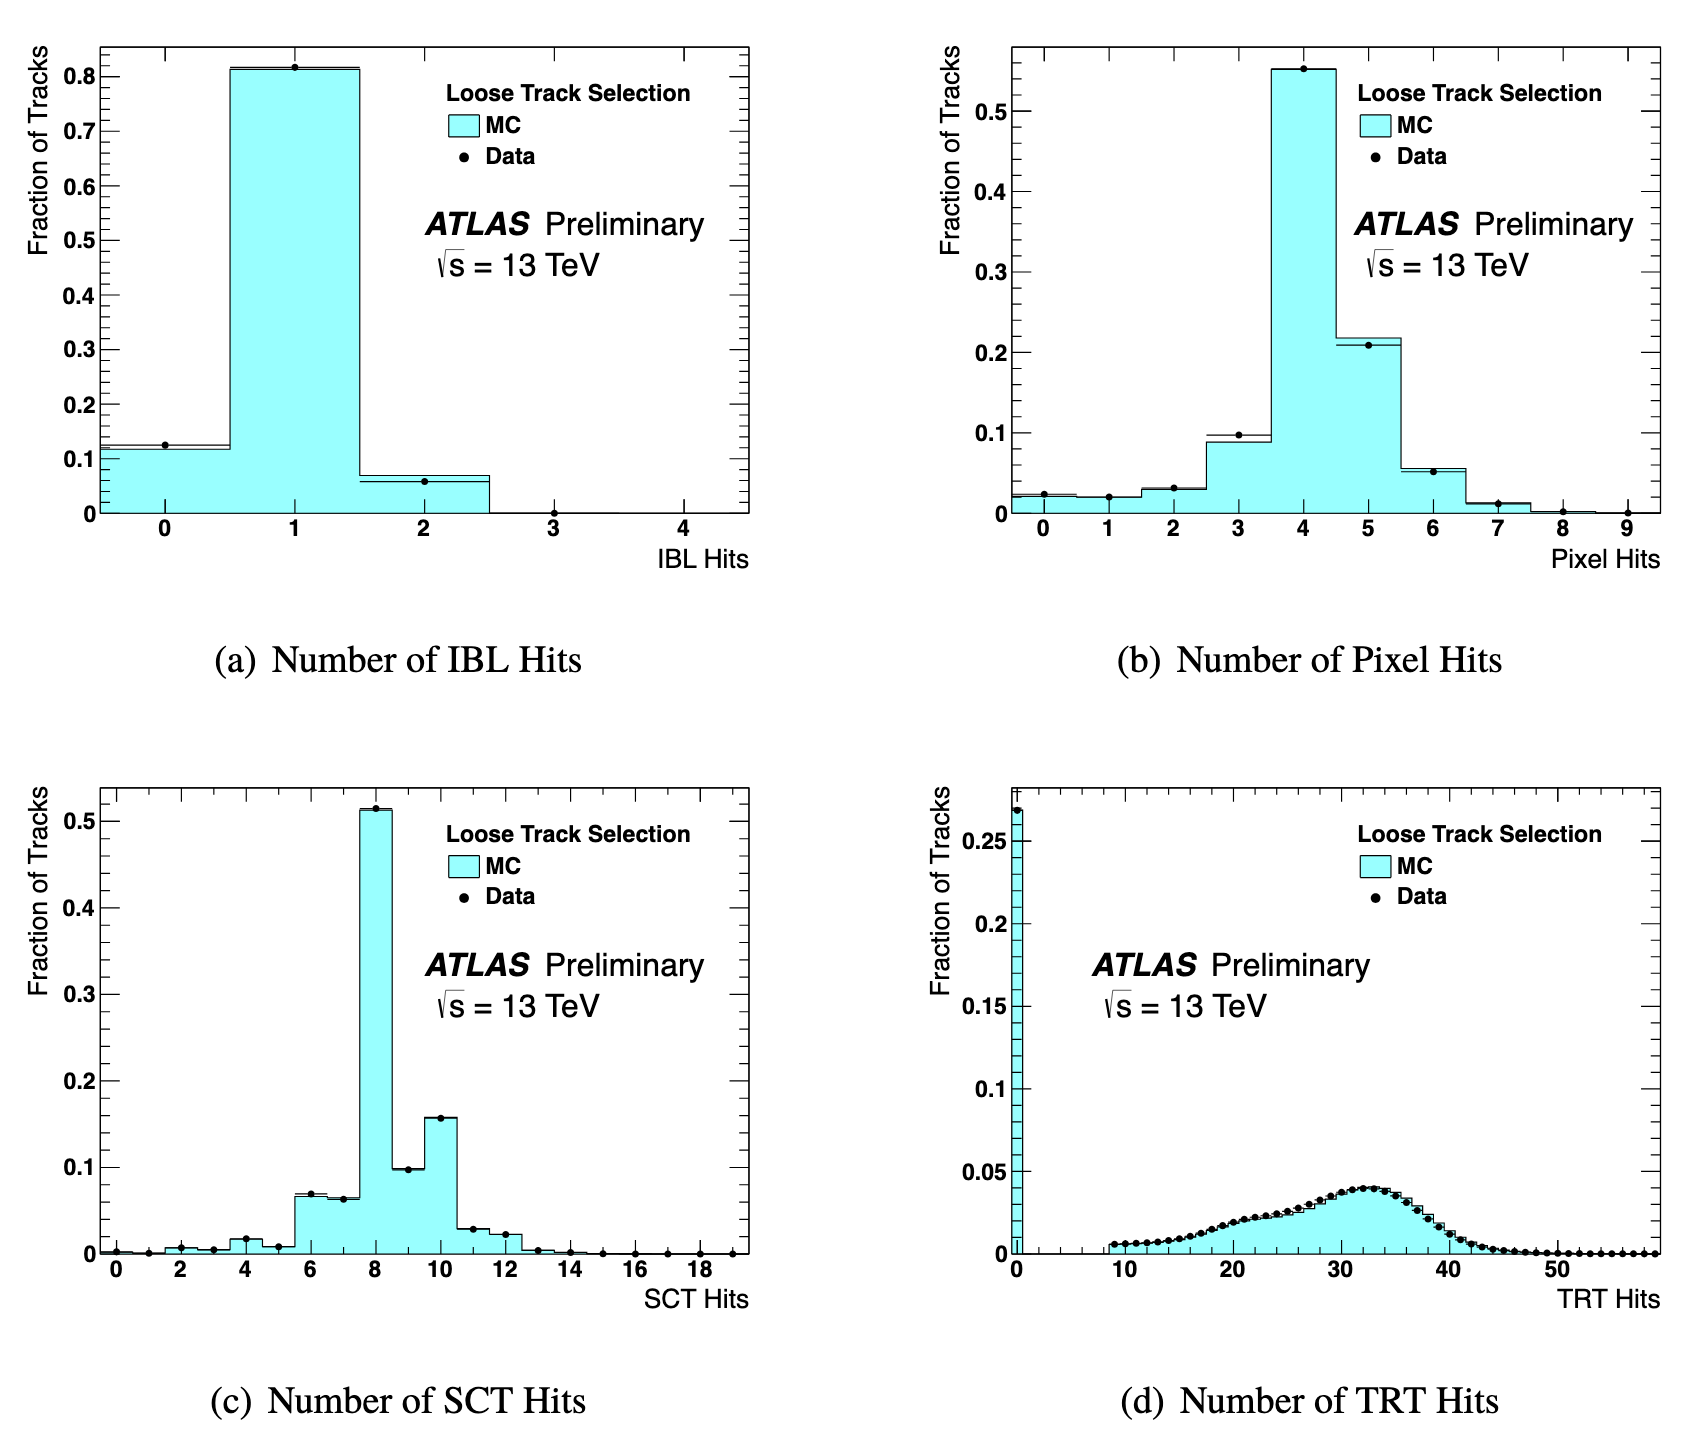
\includegraphics[width=\textwidth]{id_subdetector_hits}
	\caption{Comparison of the number of (a) IBL, (b) Pixel, (c) SCT, and (d) TRT tracking hits distributions in data and simulation for the Loose track selection. The distributions are normalized to one so that the bin contents represent track fraction. \cite{ATL-PHYS-PUB-2015-018}
	}
	\label{fig:id_subdetector_hits}
\end{figure}

The tracking procedure for ATLAS is divided into four separate stages \cite{Salzburger:2015sgq}:
\begin{enumerate}
    \item \textbf{Data Preparation and Space Point Formation}\\
        When a charged particle passes through the active silicon material of the various ID sub-detectors, it leaves behind \textit{clusters} of energy deposits resulting in raw data output spanning multiple nearby sensors.
        The first tracking stage consists of finding these connected clusters and associating them together into a single three-dimensional location.
        The difficulty of this process is compounded by the fact that nearby particle trajectories can in many cases \textit{merge} together into the same cluster.
        This is particular common in the case of high $p_T$ jets, covered in Chapter~\ref{ch:jets}.
        This necessitates the use of a neural network based cluster splitting routine for the Pixel detector.
        After clusters are identified and (potentially) split, their locations are transformed from the local sub-detector coordinate system to the global ATLAS coordinate system and referred to as \textit{space points}.
    \item \textbf{Space Point Seeded Track Finding}\\
        The process of converting space points into actual tracks begins by forming track \textit{seeds} built from triplets of space points.
        These triplets may come from any combination of space points from either of two innermost ID sub-detectors: Pixel and SCT.
        To reduce the number of potential seeds, each individual space point is restricted to appear in only a small number of seeds.
        Seeds which pass a set of loose initial requirements are passed to a \textit{track finding algorithm} which utilizes the Kalman Filter~\cite{KalmanRE} technique.
        The goal at this stage is to produce a set of \textit{track candidates}, consisting only of space points within the Pixel/SCT detectors, to pass forward to the next tracking stages.
    \item \textbf{Ambiguity Solving}\\
        At this stage, some of the track candidates may be \textit{fake} or \textit{duplicates}.
        Fake tracks result from a random combination of space points that manage to pass the loose quality requirements of the track seeding described above.
        Because space points are allowed to be shared between different track candidates, it is also possible for the same charged particle to manifest as two separate track candidates.
        At this stage it is necessary to reject as many of these fake/duplicate tracks as possible.
        The \textit{ambiguity solving algorithm} achieves this by scoring track candidates.
        Positive scores are gained by track candidates that possess unique (non-shared) space points and good fit quality from the Kalman Filter algorithm.
        Negative scores are assigned to track candidates which possess shared hits or missing hits (called \textit{holes}) in a Pixel/SCT layer where they would be expected.
    \item \textbf{TRT Extension}\\
        After passing the ambiguity resolution stage, the final set of track candidates are extended to include hits from the TRT, the outermost ID sub-detector.
        This process is only performed for track candidates within the acceptance of the TRT.
        When the TRT extension is successful, the momentum resolution is significantly improved.
\end{enumerate}

These resulting tracks are then individually fit with a $\chi^2$ minimization routine \cite{Cornelissen:2008zza} which accounts for the magnetic field strength in each region of the detector, the position error on each hit as well as the possibility of mulitple scattering. This final track fitting produces an estimate of the \textit{track parameters}.

The track selection requirements are
\begin{enumerate}
    \itemsep0em 
    \item \textbf{Loose} \begin{itemize}
        \itemsep0em 
        \item $p_T > 400$\ MeV
        \item $|\eta| < 2.5$
        \item number of silicon (IBL + Pixel + SCT) hits $\geq$ 7
        \item number of shared modules $\leq 1$
        \item number of silicon holes $\leq 2$
        \item number of pixel holes $\leq 1$
    \end{itemize}
    
    \item \textbf{Tight} \footnote{The Tight selection requirements are applied \textit{on top of} the Loose requirements.} \begin{itemize}
        \itemsep0em 
        \item if $|\eta| \leq 1.65$, number of silicon hits $\geq 9$
        \item if $|\eta| > 1.65$, number of silicon hits $\geq 11$
        \item either one IBL or next-to-innermost-Pixel-layer hit
        \item no Pixel holes
    \end{itemize}
\end{enumerate}


\section{Vertices}
In order to perform physics analysis it is vital to determine the location of the individual proton-proton collisions in each event at the ATLAS detector.
The \textit{vertex finding} algorithm is divided into four major steps which are iterated numerous times to reconstruct each vertex in the event  \cite{Borissov:2015djv}:
\begin{enumerate}
    \item 
        The arithmetic mode of the $z_0$ impact parameter for all (remaining) tracks in an event is computed in order to produce an initial \textit{seed} vertex.
    \item 
        Tracks compatible with the seed are grouped together for fitting.
    \item 
        The adaptive vertex fitting algorithm is used to estimate the position and uncertainty of the vertex.
    \item
        Remaining tracks that are incompatible with this new vertex are removed and used to repeat the entire procedure again, starting by computing a new seed.
\end{enumerate}
This vertex finding algorithm is tuned to balance two competing difficulties: (1)~Splitting a real vertex into multiple reconstructed vertices and (2) merging two proton-proton interactions into the same reconstruction vertex. 
The vertex with the largest $\sum p_T^2$ for all associated tracks is termed the hard-scatter vertex. In general all physics analysis work considers only objects associated to this vertex, while all other reconstructed vertices are considered to be the result of pile-up.

\section{Electrons}
Electrons interact primarily with the EM calorimeters (described in Sec.~\ref{sec:calorimeters}) by leaving a signature in groups of neighboring cells.
The reconstruction of electrons is performed by matching reconstructed tracks from the ID with these calorimeter deposits.
Electron reconstruction in the central region of the ATLAS detector ($|\eta| < 2.47$) proceeds in several steps \cite{ATLAS-CONF-2016-024}:

\begin{enumerate}
    \item \textbf{Seed-Cluster Reconstruction}\\
        A $3 \times 5$ sliding window\footnote{The sliding window grid has has units of $0.025 \times 0.025$ in $(\eta, \phi)$ space, which corresponds to the granularity of the middle layer of the EM calorimeter.} is used to search for electron cluster \textit{seeds}.
        For position of the sliding window the total energy is summed across all longitudinal layers for each contained cell, forming a so-called \textit{tower}.
        If the sum of transverse energy from the towers in the window is greater than 2.5 GeV, a seed cluster is formed.
        If the seed cluster passes certain quality requirements a \textit{Region of Interest} (ROI) is specified surrounding the location of the cluster.
    \item \textbf{Track Reconstruction}\\
        Several intricacies of the track-fitting (described in Section \ref{sec:tracking}) are modified in order to assist with the reconstruction of electrons.
        By default the ATLAS tracking procedure assumes tracks correspond to particles with an energy loss model corresponding to pions.
        However, this model can be substituted for an alternative model that allows for up to 30\% energy loss at each intersection of the track with the ID material.
        This alternative model accounts for the possibility of bremsstrahlung.
        During the execution of the tracking algorithm, if a track seed with $p_T > 1$ GeV cannot be extended into a full track with at least seven hits using the pion energy loss model, a second attempt is performed using the electron energy loss hypothesis.
        Furthermore, if a track candidate is produced with the pion hypothesis but fails the final Global $\chi^2$ track fit, it is then refit with the electron hypothesis.
        Tracks utilizing the electron hypothesis are tagged as such and utilized in the next steps of the electron reconstruction process.
    \item \textbf{Electron-Specific Track Fit}\\
        The tracks obtained in the previous step are then loosely matched to the EM clusters based on their separation in the $\eta-\phi$ plane.
        In order to perform this matching the trajectory of the track is extended into the center of the EM calorimeter.
        Tracks with $\geq 4$ pixel layer hits which are loosely associated to electron clusters are refit using an optimized Gaussian Sum Filter (GSF) \cite{ATLAS-CONF-2012-047} which is specialized to account for non-linear bremsstrahlung effects.
        A similar but stricter matching as the one described above is performed again with the refitted track.
    \item \textbf{Electron Candidate Reconstruction}\\
        If multiple tracks fulfill the matching criteria for the same EM cluster, one of them is chosen as the \textit{primary} track.
        The choice is based upon a number of criteria: (1) cluster-track distance in the $\eta-\phi$ plane, (2) number of hits in the Pixel detector and (3) the presence of a hit in the first silicon layer.
        If a cluster is not associated to any tracks at this point, it is removed and considered as a photon candidate.
        The efficiency of electron identification is shown in Figure~\ref{fig:electron_eff_Zee}.
        The energy of the clusters is then calibrated to match that of the original electron energy using multivariate techniques based on simulated MC samples \cite{Aaboud:2018ugz}.
        The four-momentum of the electron is then computing using the energy information from the final calibrated energy of the cluster and directional information ($\eta, \phi$) from the best track matched to the original seed cluster.
\end{enumerate}

\begin{figure}
	\centering
	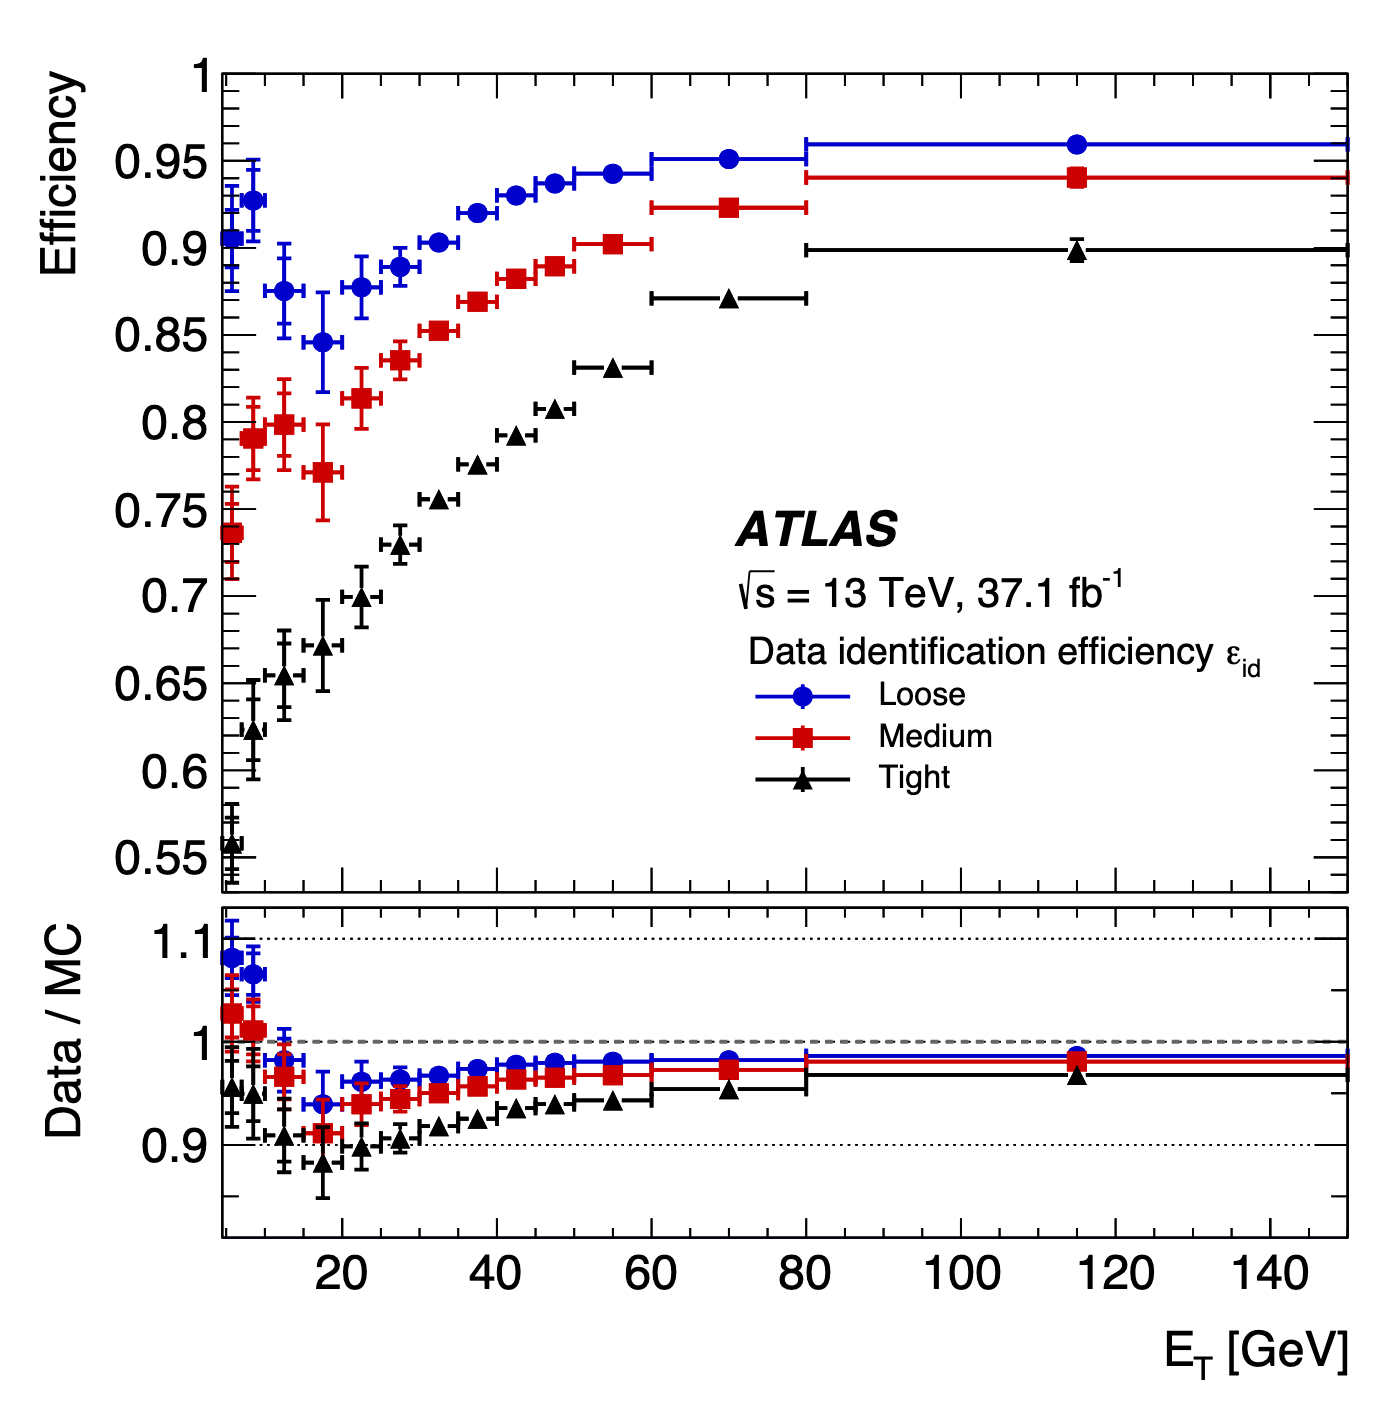
\includegraphics[width=0.65\textwidth]{electron_eff_Zee}
	\caption{
	    The electron identification efficiency in $Z \rightarrow ee$ events in data as a function of transverse energy ($E_T$) for the Loose, Medium, and Tight working points.
	    The efficiency in data is obtained by applying data-to-simulation efficiency ratios that are measured in $J/\psi \rightarrow ee$ and $Z \rightarrow ee$ events to the $Z \rightarrow ee$ simulation.
	    \cite{Aaboud:2018ugz}
	}
	\label{fig:electron_eff_Zee}
\end{figure}

\section{Muons}
Muons are minimum ionizing particles that interact weakly with the ATLAS calorimeter system, depositing approximately 3-4 GeV there on average \cite{Lenzi_2010}.
Thus, as discussed in Section \ref{sec:muon_spectrometer}, muons are reconstructed primarily by combining tracking information from the ID and MS.
Within the ID, tracks from muons are not treated any differently than any other type of charged particle.
Within each sub-detector region of the MS (MDTs, CSCs, etc) a Hough transform \cite{10.1016/S0734-189X(88)80033-1} is used to search for hits aligned in the bending plane of the detector (produced by the magnetic field) and produce muon \textit{track candidates}.
Track candidates are formed by combining hits from different track segments via a combinatorial search \cite{Aad:2016jkr}.
After this an overlap removal algorithm is run to find the most optimal track assignment.
The final track candidates are fit with a global $\chi^2$ minimization algorithm, similar to ID track reconstruction.
Finally, a hit recovery and track re-fit are performed if necessary.

Four types of muons emerge from the reconstruction process, depending on which sub-detectors are involved:
\begin{itemize}
    \item \textbf{Combined Muons (CB)}\\
        A global fit is used to combine hits form both the ID and the MS while accounting for energy loss in the calorimeter.
        The track from the MS is used as the primary starting point and extrapolated inward and matched to a single ID track.
        These are the most common types of reconstructed muons used in physics analyses, as they have the highest purity and best kinematic resolution.
    \item \textbf{Segment-Tagged Muons (ST)}\\
        Like the CB muons, ST muons are constructed by combining ID and MS hits.
        However, in the case of ST muons, a local track segment from either the MDT or CSC chambers is used in place of a full MS track.
        This strategy is necessary for reconstructing muons which cross only one layer of the MS chambers.
        This typically occurs when the muon possesses low $p_T$ and passes through only one region of the MS.
    \item \textbf{Calorimeter-Tagged Muons (CT)}\\
        In the case where an ID track can be matched to a deposit in the calorimeter system which is compatible with a minimum ionizing particle, some muons can be reconstructed in regions where the MS has low acceptance around $|\eta| \approx 0$.
    \item \textbf{Extrapolated Muons (ME)}\\
        In the region beyond the ID acceptance but still within the MS acceptance ($2.5 < |\eta| < 2.7$) some muons can still be reconstructed by utilizing only MS tracks. A loose requirement is placed to ensure the MS track points towards the IP.
\end{itemize}

As with electrons, muon candidates are categorized according to purity: ``Loose'', ``Medium'', and ``Tight''.
The muon reconstruction efficiency at ATLAS is nearly 100\%, as seen in Figure~\ref{fig:muon_efficiency}.

\begin{figure}
	\centering
	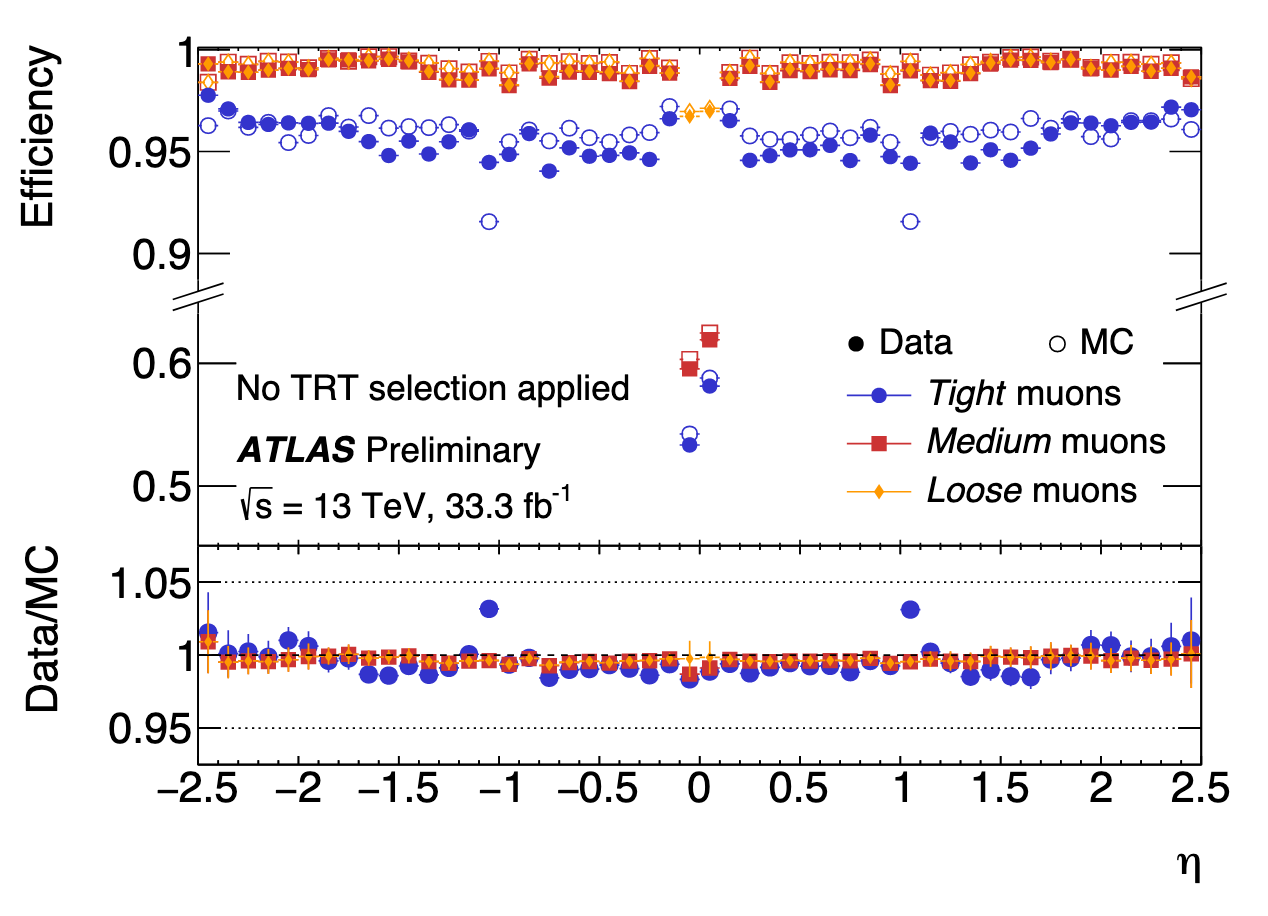
\includegraphics[width=0.85\textwidth]{muon_efficiency}
	\caption{
	Muon reconstruction efficiencies for the Loose/Medium/Tight identification algorithms measured in $Z\rightarrow \mu\mu$ events as a function of the muon pseudorapidity ($\eta$) for muons with $p_T > 10$\; GeV. The prediction by the detector simulation is depicted as open circles, while filled dots indicate the observation in collision data with statistical errors.
	The bottom panel shows the ratio between expected and observed efficiencies: the effiency scale factor.
	The errors in the bottom panel show the quadratic sum of statistical and systematic uncertainty.
	    \cite{Marchese:2018vrd}
	}
	\label{fig:muon_efficiency}
\end{figure}